\documentclass[a4paper, 12pt]{article}
\usepackage[a4paper, total={6in, 8in}]{geometry}
\geometry{
	a4paper,
	left = 1.5 cm,
	right = 1.5 cm,
	top = 2cm,
}
\usepackage[T1]{fontenc}
\usepackage{pythontex}
\usepackage{hhline}
\usepackage{array,booktabs}
\newcolumntype{M}[1]{>{\centering\arraybackslash}m{#1}}
\usepackage[table]{xcolor}
\usepackage{caption}
\usepackage{makecell}
\usepackage{lipsum}
\usepackage{pifont}
\usepackage{amssymb}
\usepackage{amsmath}
\usepackage[utf8]{inputenc}
\usepackage[italian]{babel}
\usepackage{graphicx}
\graphicspath{ {./images/} }
\usepackage{spverbatim}
\usepackage{float}
\usepackage{url}
\usepackage{xstring}
\usepackage{hyperref}
\usepackage{xcolor}
\definecolor{linkcolor}{RGB}{1,1,87}
\hypersetup{
    colorlinks,
    citecolor=black,
    filecolor=black,
    linkcolor=linkcolor,
    urlcolor=blue
}
\usepackage{fancyvrb,newverbs,xcolor}
\definecolor{cverbbg}{gray}{0.93}
\definecolor{cellcolor}{RGB}{165,194, 242}
\usepackage{xifthen}
\usepackage{multirow}
\usepackage{adjustbox}


\newcommand{\checkbox}[0]{\item[$\square$]}
\newcommand{\done}[0]{\item[$\text{\rlap{$\checkmark$}}\square$]}

\newcommand{\sysroot}[0]{\key{\%SYSTEMROOT\%}}
\newcommand{\makesub}[1]{%
  \saveexpandmode\noexpandarg
  \StrSubstitute{#1}{\_}{_}[\temp]%
  \restoreexpandmode%
}

\newcommand{\target}[1]{%
  \makesub{#1}%
  \hypertarget{\temp}{}%
}

\newcommand{\attach}[1]{%
  \makesub{#1}%
  \hyperlink{\temp}{\emph{#1}}%
}
\newcommand{\attachcode}[1]{%
  \makesub{#1}%
  \hyperlink{\temp}{\code{#1}}%
}
\newcommand{\attachkey}[1]{%
  \makesub{#1}%
  \hyperlink{\temp}{\key{#1}}%
}

\newcommand{\code}[1]{\colorbox{cverbbg}{\texttt{\StrSubstitute{#1}{_}{\_}}}}

\newcommand{\linux}{\textit{Linux}}
\newcommand{\win}{\textit{Windows}}
\newcommand{\nota}[1]{\textbf{Nota}: #1}
\newcommand{\memo}[1]{\textbf{Memo}: #1}
\newcommand{\esempio}[1]{\textbf{Esempio}: #1}
\newcommand{\tbs}{\textbackslash}
\newcommand{\ghidra}{\emph{Ghidra}}
\newcommand{\ollydb}{\emph{OllyDbg}}
\newcommand{\Null}{\code{NULL}}
\newcommand{\dll}{\emph{DLL}}
\newcommand{\api}{\emph{API}}
\newcommand{\key}[1]{\texttt{\StrSubstitute{#1}{_}{\_}}}

\newcommand{\paramtable}[2][]{%
\ifthenelse{\isempty{#2}} {\input{|"/home/luca/Scrivania/MA/homeworks/homework-04/report/scripts/generate_param_table.py '#1'"}} {\input{|"/home/luca/Scrivania/MA/homeworks/homework-04/report/scripts/generate_param_table.py '#1' '#2'"}}%
}
\newcommand{\image}[1]{\input{|"/home/luca/latex_scripts/add_image.py '#1'"}}

\newcommand{\eax}[0]{\key{EAX}}
\newcommand{\ebx}[0]{\key{EBX}}
\newcommand{\ecx}[0]{\key{ECX}}
\newcommand{\edx}[0]{\key{EDX}}
\newcommand{\ebp}[0]{\key{EBP}}
\newcommand{\esp}[0]{\key{ESP}}
\newcommand{\esi}[0]{\key{ESI}}
\newcommand{\edi}[0]{\key{EDI}}
\newcommand{\struct}[3]{%
\begin{tabular}{|c|c|}%
\hline%
following byte address & #1 \\%
\hline%
current byte & #2 \\%
\hline%
remaining bits & #3 \\%
\hline%
\end{tabular}%
}

\newenvironment{myverb}
 {\SaveVerbatim{cverb}}
 {\endSaveVerbatim
  \flushleft\fboxrule=0pt\fboxsep=.5em
  \colorbox{cverbbg}{%
    \makebox[\dimexpr\linewidth-2\fboxsep][l]{\BUseVerbatim{cverb}}%
  }
  \endflushleft
}

\setcounter{tocdepth}{4}
\setcounter{secnumdepth}{4}
\setlength\parindent{0pt}

\begin{document}\sloppy
  
\title{
  \textbf{
    \emph{Relazione homework 4}
  }
}  
\author{Luca Mastrobattista\\Matricola: 0292461}
\date{}
\maketitle

\tableofcontents
\newpage
\part{Traccia dell'homework}
\target{consegna}
\section{Testo}
Analizzare il programma eseguibile hw4.ex\_ contenuto
nell'archivio hw4.zip (password: "AMW21").
Determinare ogni possibile informazione riguardo alle
funzionalita' del programma, riassumendole in un documento
che riporti anche la metodologia adottata ed i passi logici
deduttivi utilizzati nel lavoro di analisi.\\
ATTENZIONE: IL MALWARE E' REALE E PUO' PROVOCARE DANNI AI
SISTEMI INFORMATICI SE NON OPPORTUNAMENTE CONTROLLATO E
MONITORATO.

\section{Scadenza}
Tre giorni prima della data d'appello in cui si
intende sostenere l'esame orale.

\section{Consegna}
Documento in formato PDF inviato come allegato ad
un messaggio di posta elettronica all'indirizzo del docente
("$<$cognome$>$@uniroma2.it"), con subject:
"[AMW21] HW4: $<$matricola studente$>$"


\newpage
\part{Analisi}

\section{Basic static (code) analysis}
Utilizzando il comando \code{strings} da terminale \linux{}, si nota come le stringhe sembrino essere cifrate. È ragionevole pensare che il programma sia stato impacchettato. Una conferma la troviamo analizzando il file con il tool \textit{PEiD}:\\
\begin{minipage}{0.4\textwidth}
\begin{figure}[H]
\centering 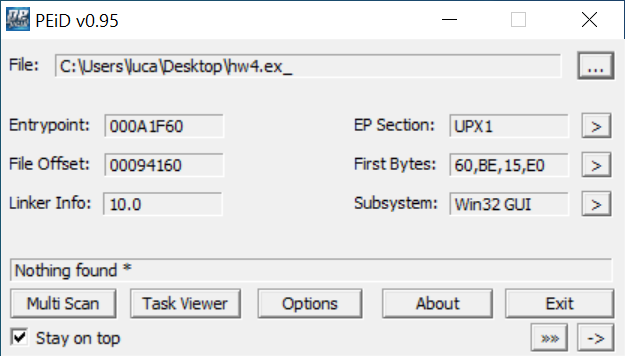
\includegraphics[width=\textwidth]{peid}
\end{figure}
\end{minipage}\hfill
\begin{minipage}{0.4\textwidth}
\begin{figure}[H]
\centering 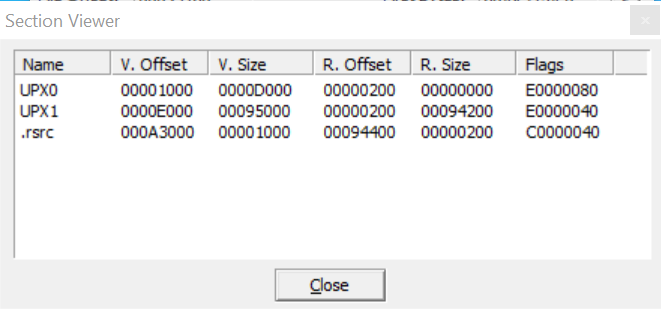
\includegraphics[width=\textwidth]{peid2}
\end{figure}
\end{minipage}\\

Nella sezione \key{EP Section} notiamo \key{UPX1}: significa che l'eseguibile è stato effettivamente impacchettato con il \textit{packer} open source \key{UPX}, che viene però identificato solo dopo aver eseguito una \textit{Deep scan}: \key{UPX 0.89.6 - 1.02 / 1.05 - 2.90 -> Markus \& Laszlo}. Si può quindi scompattare automaticamente eseguendo \code{upx -d hw4.ex_ -ounpacked.ex_} sul sistema host. Il file ottenuto è leggermente più grande del file originale: potrebbe aver funzionato. Eseguendo nuovamente il comando \code{strings} sul file \textit{unpacked.ex\_} si possono leggere molte stringhe note, come ad esempio \key{"kernel32.dll"}. Il file ottenuto, però, non risulta eseguibile. 

\section{Basic dynamic (behaviour) analysis}
Eseguendo il malware su una macchina virtuale \win{} non collegata alla rete, si può osservare che questo si tratta in realtà di un \textit{ransomware}: dopo aver terminato la sua esecuzione, vengono creati due nuovi file, un file \key{asasin.htm} e un file \key{asasin.bmp}, che riportano la stessa scritta; si tratta delle istruzioni da seguire per ottenere la chiave per decifrare i dati; l'immagine viene anche impostata come sfondo. Inoltre, ogni file che viene criptato dal malware viene convertito in un file con estensione \key{.asasin}. Si nota inoltre che alla fine dell'esecuzione il malware non è più presente sul desktop: con buona probabilità si è eliminato dopo aver completato l'esecuzione.

\subsection{Definizione chiara degli obiettivi}
Nella \attach{consegna} viene richiesto di determinare ogni possibile informazione sulle funzionalità del programma. Tuttavia questo malware, con molta probabilità, sarà molto grande e una delle lezioni più importanti del corso è stata quella di eseguire l'analisi del malware avendo chiaro un obiettivo, perché non si può riuscire a capire tutto in tempi ragionevoli. Per questo motivo, con le informazioni note a questo punto e considerando che un \textit{ransomware} ha un comportamento tale per cui in genere non cerca di rimanere nascosto nel sistema, l'analisi verrà ristretta a quelli che sembrano essere gli aspetti principali:



{
	\definecolor{partscolor}{RGB}{12,4,128}
	\hypersetup{
	colorlinks,
    	citecolor=black,
    filecolor=black,
    linkcolor=partscolor,
    urlcolor=blue
	}

\begin{itemize}
\done \textbf{\attach{Ricostruzione del codice}}: all'inizio il malware ricostruirà il codice malevole. Ricercare l'\textit{entry point}, con conseguente ottenimento dell'eseguibile non impacchettato


\item Cifratura:
	\begin{itemize}
	\done \hyperlink{RSA key}{\emph{\textbf{Come viene recuperata la chiave RSA}}}
	\done \hyperlink{Cifratura}{\textbf{\emph{Quali files vengono cifrati e con quale chiave AES}}}
	\end{itemize}

\item Generazione dei file sul desktop: 
	\begin{itemize}
	\done \hyperlink{files asasin}{\textbf{\emph{Come recupera il testo dei file} \key{asasin.*} \emph{sul desktop}}}
	\done \hyperlink{files asasin generation}{\textbf{\emph{come genera i file} \key{asasin.*}}}
	\end{itemize}


\done \textbf{\attach{Auto-eliminazione}}: come fa il malware a eliminarsi, se è effettivamente così

\done \textbf{\attach{Meccanismi anti-debugging e anti-disassbler}}: quali meccanismi di anti-debugging e anti-disassemblaggio sono presenti
\end{itemize}
}


\target{Ricostruzione del codice}
\part{Ricostruzione del codice}
Cerchiamo per prima cosa di recuperare l'eseguibile \textit{unpacked}, in modo da poter seguire il flusso contemporaneamete con debugger e disassemblatore. Come detto, usando \textit{upx} il programma di output non risulta eseguibile. Si procede quindi in altri modi.

\section{Ricerca dell'OEP}
Utilizzando \ghidra{} per identificare i vari \key{JMP} dell'eseguibile impacchettato, notiamo che ce n'è qualcuno veramente grande:
\begin{figure}[H]
\centering 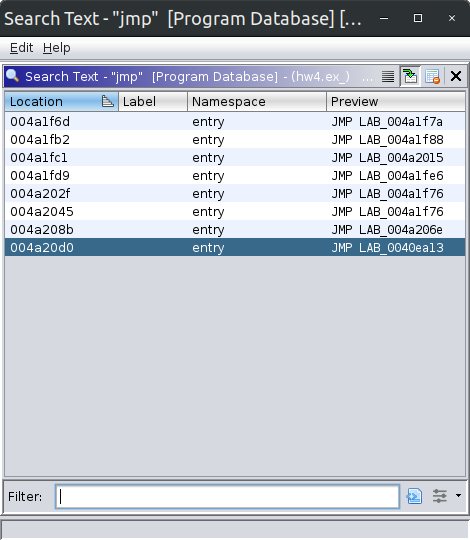
\includegraphics[scale=0.4]{jumps}
\end{figure}

In particolare, il salto evidenziato è veramente grande, e potrebbe essere effettivamente il nostro \textit{tail jump}. Tuttavia, per una conferma, sfruttiamo \ollydb{}: il codice, infatti, utilizza nell'\textit{entry point} dello stub l'istruzione \code{PUSHAD} e si può quindi verificare che i registri verranno recuperati prima del salto evidenziato. \\
Il codice si interrompe proprio prima di quel salto: si può concludere che l'\textit{OEP} sia effettivamente all'indirizzo \key{0x0040ea13}. Utilizzando il plugin \textit{OllyDump}, si prova a questo punto a eseguire il dump di memoria con tutti e 3 i metodi: 
\begin{enumerate}
\item ricreando la \textit{IAT} tramite istruzioni di \code{JMP} e \code{CALL}
\item ricreando la \textit{IAT} tramite il nome delle \api{} invocate
\item senza ricreare la \textit{IAT}
\end{enumerate}
Entrambi i primi due metodi ricostruiscono l'\textit{IAT} correttamente: provando a lanciare gli eseguibili ottenuti, infatti, si verifica lo stesso comportamento del malware originale. Analizzandolo con \ghidra{}, però, il codice non viene decompilato: il dump è stato fatto prima che l'eseguibile fosse de-impacchettato completamente, ma comunque è stato decodificato un primo step. Cercando ulteriori salti all'interno del nuovo eseguibile, ce ne sono solo 3: uno è molto breve e gli altri due saltano a contenuti all'interno di aree di memoria che staticamente non sono identificabili. Si procede eseguendo lo stub con debugger per cercare l'OEP reale.

\section{Advanced analysis}
All'indirizzo \key{0x0040699a} si invoca indirettamente la funzione \code{VirtualAlloc}, allocando \key{0x688} bytes, cioè 1672. Questa memoria viene scritta nelle successive istruzioni, decodificando \key{0x688} bytes a partire dall'indirizzo \key{0x00496000}. Il codice appena scritto viene poi invocato. 

\subsection{Zona della prima VirtualAlloc}
Il codice eseguito in questa zona ha come obiettivo quello di giocare con i bytes della \dll{} \key{kernel32.dll} per ottenere le seguenti stringhe ASCII:
\bigskip

\begin{minipage}{0.27\textwidth}
\begin{itemize}
\item \key{LoadLibraryA}
\item \key{GetModuleHandleA}
\item \key{GetProcAddress}
\item \key{VirtualProtect}
\item \key{VirtualAlloc}
\item \key{VirtualFree}
\end{itemize}
\end{minipage}
\begin{minipage}{0.36\textwidth}
\begin{itemize}
\item \key{CloseHandle}
\item \key{CreateToolhelp32SnapshotA}
\item \key{GetModuleFileNameA}
\item \key{CreateFileA}
\item \key{SetFilePointer}
\item \key{ReadFile}
\end{itemize}
\end{minipage}
\begin{minipage}{0.33\textwidth}
\begin{itemize}
\item \key{GetCurrentProcessId}
\item \key{Module32First}
\item \key{Module32Next}
\item \key{GetProcessHeap}
\item \key{WaitForSingleObject}
\item[]
\end{itemize}
\end{minipage}
\bigskip

Dopo aver generato le stringhe, si genera un'altra zona di memoria con un'altra \code{VirtualAlloc} della stessa dimensione di quella in cui attualmente sta eseguendo, copiandovi all'interno gli stessi bytes; le due zone differiranno solo per i bytes che costituiscono le stringhe. Per saltarci dentro, però, non c'è nessuna \code{CALL} o \code{JMP}, ma si sfrutta il funzionamento dell'istruzione \code{RET}: si mette infatti sulla cima dello stack un indirizzo interno a questa zona appena creata e, quando si eseguirà \code{RET}, si riprenderà il flusso da quell'indirizzo.

\subsection{Zona della seconda VirtualAlloc}
In questa zona di memoria, il malware decodifica le varie sezioni con un meccanismo basato sulla rotazione dei bits scrivendo il risultato in una zona di memoria di \key{0x83a00} bytes, allocata con una nuova \code{VirtualAlloc}. Dopo la scrittura, vengono caricate molte funzioni attraverso l'invocazione di \code{LoadLibrary}. Si continua accedendo alla struttura dati \key{InLoadOrderList} della struttura \key{PEB_LDR_DATA}, ma non viene usata per cercare i nomi delle varie \dll{}: si accede infatti al campo all'offset \key{0x1c} che, su \href{http://undocumented.ntinternals.net/}{undocumented NTinternals}, viene chiamato \key{EntryPoint}; questo campo è sostituito con l'indirizzo \key{0x402d8f}. Abbiamo trovato l'\key{OEP}, ma nessuno degli eseguibili ottenuti dal dump fatto con \textit{OllyDump} non risultano lanciabili: la \textit{Import Address Table} non è stata ricostruita correttamente. Si può però procedere eseguendo analisi statica avanzata e dinamica avanzata in parallelo. \\

\nota{all'interno della funzione \key{entry}, c'è solo una funzione a cui \ghidra{} non riesce a dare un nome tra quelle invocate: \attachcode{FUN_0042c820}, che si tratta quindi del \code{main} del processo.}

\hypertarget{RSA key}{}
\hypertarget{files asasin}{}
\part{Ottenimento della chiave RSA e dei files asasin.*}
\target{FUN\_0042c820}
\target{FUN\_0042c820\_main}
\subsection{FUN\_0042c820\_main}
La funzione invoca \attachcode{FUN_00477050_generate_key_and_files} e, se non ritorna 0, si memorizza l'area di memoria restituita nella variabile globale \key{DAT_004831f8_key_and_files_virtual_alloc_address}, che pare essere una struttura di tipo \attachkey{rsa_and_file_data_struct}. Si invoca poi \attachcode{FUN_00429ea0_start_the_job} prima di terminare.\\

Quindi, possiamo pensare alla struttura del \key{main} come una semplice funzione che ne invoca altre due: la prima recupera il codice del file \key{htm}, il testo che verrà mostrato nell'immagine \key{.bmp} e la chiave RSA, l'altra utilizza questi contenuti per cifrare e generare i files.


\target{FUN\_00477050\_generate\_key\_and\_files}
\subsection{FUN\_00477050\_generate\_key\_and\_files}
In questa funzione avviene una nuova invocazione di \code{VirtualAlloc} di \key{0xb07} bytes, che vengono scritti ancora decodificandone altri con un meccanismo a rotazione di bits. In questa funzione, c'è anche un accesso a \hyperlink{fs30}{\key{FS:[0x30]}} per controllare se è attivo un debugger. Una ulteriore \code{VirtualAlloc} di \key{0x6494} bytes crea un'area di memoria che viene poi riempita nella funzione \code{FUN_0046e940_fill_virtualAlloc_area_with_RSA_key_and_file_content}. I bytes scritti vengono recuperati decodificandone altri: possiamo concludere che queste informazioni risultano \textit{hard-coded} all'interno dell'eseguibile, ma sono codificate e quindi risultano trasparenti a un'analisi statica. \\
L'area di memoria che contiene questi dati è stata interpretata come una struttura di tipo \attachkey{rsa_and_file_data_struct}.

\target{FUN\_00429ea0\_start\_the\_job}
\subsection{FUN\_00429ea0\_start\_the\_job}
\nota{da qui in poi la funzione fa un pesante uso delle strutture \attachkey{buffer_handler_ASCII} e \attachkey{buffer_handler_UNICODE}.}\\

La funzione invoca \code{SetErrorMode} con parametro \key{ErrorMode} impostato a \key{0x8003}: questo valore corrisponde alla combinazione \key{SEM_FAILCRITICALERRORS | SEM_NOGPFAULTERRORBOX  | SEM_NOOPENFILEERRORBOX}; con questa invocazione, quindi, si previene la creazione di:
\begin{itemize}
\item \key{Critical-error-handler message box}: l'eventuale errore viene inviato al processo stesso
\item \key{Windows Error Reporting Dialog}
\item \key{Message Box} per fallimento dell'\api{} \code{OpenFile}
\end{itemize}

Successivamente viene invocata \code{SetUnhandledExceptionFilter}, con cui si imposta la \textit{default routine} per la gestione delle eccezioni alla funzione \code{FUN_0041f820_unhandled_default_routine}. Si continua mettendo in \key{EAX} il valore del campo \key{sleepTime} della struttura dati \attachkey{rsa_and_file_data_struct} e viene moltiplicato per 1000$_{10}$; il risultato viene usato come parametro di una invocazione di \code{Sleep}: si dorme per 12 secondi.\\

Vengono poi invocate le funzioni \code{FUN_0041f680_get_path_name_struct} e \code{FUN_0041f560_get_tmp_path_in_struct}, per ottenere delle strutture \attachkey{buffer_handler_UNICODE} che contengano nel loro buffer rispettivamente il path completo del file eseguibile e quello della cartella di sistema \key{Temp}. \\

Si controlla il campo \key{change_in_svchost} della struttura \attachkey{rsa_and_file_data_struct} e, se non è 0, il codice continua copiando l'eseguibile nella cartella \key{Temp}, cambiandone il nome in \key{svchost.exe} ed eseguendolo in un nuovo processo dal \key{cmd}; in questo caso si continua rilasciando le risorse per poi terminare. Se invece quel campo vale 0, si continua invocando \code{GetVolumeNameForVolumeMountPoint} con parametro \key{lpszVolumeMountPoint = "C:\tbs{}"}. La parte numerica del valore restituito viene usata come input per la funzione\code{FUN_00431440_get_half_md5_struct}, al cui interno viene ottenuto un \key{CSP} (\textit{Cryptographic Service Provider}) che viene usato per eseguire una \key{MD5} sul parametro in input. Tuttavia viene restituita solo la prima metà dell'\textit{hash}, in versione stringa, all'interno del buffer di una struttura \attachkey{buffer_handler_ASCII}.\\


%
% Se invece quel campo vale 0, si continua invocando \code{FUN_00431440_get_half_md5_struct}, al cui interno viene ottenuto un \key{CSP} (\textit{Cryptographic Service Provider}) e viene usato per generare una \key{MD5} a partire dalla parte numerica dell'output della funzione \code{GetVolumeNameForVolumeMountPoint}, invocata con parametro \key{lpszVolumeMountPoint = "C:\tbs{}"}.\\

Nel mio caso, l'input per la \textit{hash function} è il valore numerico di \key{\tbs{}\tbs{}?\tbs{}Volume\{1c6d0bcb-0000-0000-0000-300300000000\}\tbs{}} compresa di parentesi graffe, cioè \key{\{1c6d0bcb-0000-0000-0000-300300000000\}}. L'output dell'\key{MD5} sarebbe \key{0xa2 0x46 0x0d 0xcc 0xbd 0x90 0x3c 0x0d 0x5d 0x8c 0xa1 0x6d 0x4e 0x37 0xdf 0x9d}, e perciò la struttura restituita memorizzerà la stringa \key{A2460DCCBD903C0D}.\\

Come si può notare, il buffer della struttura contiene comunque una stringa di 16 caratteri, cioè 128 bit: è la dimensione di una \textit{hash} \key{MD5}. Questa struttura viene memorizzata in una variabile globale: \key{DAT_00481fb4_half_md5_struct}, ma non risulta funzionale ai fini dell'encryption. Viene però usata dalla successiva invocazione di \code{FUN_004270f0_search_for_atom}, una sorta di wrapper per \code{GlobalFindAtomA} e \code{FindAtomA} sulla stringa \key{$\sim\sim\sim$<half_hash>$\sim\sim\sim$}: potrebbe essere una sorta di firma del malware perché, nel caso la trovi, l'esecuzione termina rilasciando risorse. \\
Si continua poi generando un'altra struttura ASCII, il cui buffer contiene 16 caratteri costruiti a partire dalle informazioni di sistema, come la lingua e le metriche di sistema. Provando a lanciare l'eseguibile più volte, questa stringa è sempre uguale sul mio computer: \key{BIDM66TH652055MZ} e viene infatti usati come \key{id} per il pc su cui gira. Questa stringa va a sostituire quella generata precedentemente all'interno della struttura \key{DAT_00481fb4_half_md5_struct}.\\

\nota{questa stringa non è ottenuta con un'invocazione crittografica}\\

Il codice continua creando una struttura ASCII per il testo dell'immagine bitmap, una per il codice html e una per la chiave RSA. \\
Il testo da inserire nell'immagine, così come il testo del file html, contengono molte volte la stringa \key{FF000000000000FF}: tutte le occorrenze vengono quindi sostituite con il contenuto di \key{DAT_00481fb4_half_md5_struct}, cioè la stringa costruita a partire dalle statistiche del pc.\\

Vengono poi creati due thread all'interno di un loop con la funzione
\code{CreateThread}, che prendono come routine di partenza la funzione \attachcode{FUN_00429b40_thread_func}. La \textit{thread procedure} riceve un parametro di tipo \key{buffer_handler_UNICODE}, diverso per i due thread: 
\image{thread_params;0.4}
{\centering \textit{I due thread verranno riferiti rispettivamente come \key{thread 1} e \key{thread 2}}\par}
\bigskip

Viene creato un thread per ogni volume del sistema, recuperati precedentemente con l'invocazione di una funzione che non è stata però approfondita. Ogni thread creato si occuperà della cifratura dei dati contenuti nel volume specificato dal buffer della struttura passata, mentre il thread principale si mette in attesa della loro terminazione. \\

Dopo averli attesi si invoca \code{FUN_004273c0_add_atom_to_local_and_global_table}, al cui interno viene costruita la stringa \key{$\sim\sim\sim$<hash_id>$\sim\sim\sim$}, usata poi come parametro di \code{AddAtomA} e \code{AddGlobalAtomA}: viene registrata l'hash descrittiva dell'utente anche all'interno della \textit{atom table} di sistema: si tratta effettiamente di una firma lasciata dal malware. \\

A questo punto il ransomware inizia a fare confusione: si invoca infatti la funzione \attachcode{FUN_00425870_create_desktop_files_and_open_them}, al cui intervo vengono generati i file bmp e htm, che vengono poi aperti da una invocazione di \code{ShellExecuteW}. 

\target{Auto-eliminazione}
\paragraph*{Auto-eliminazione}
La funzione, infine, invoca 	\code{FUN_00431de0_exit_wrapper} in cui, prima di terminare, il file eseguibile viene spostato nella cartella \key{Temp} sotto forma di file temporaneo, il cui nome è generato a partire dal prefisso \key{sys}. Questo nuovo file viene inoltre marcato come file da eliminare dal sistema al prossimo riavvio.

\target{Cifratura}
\part{Encryption}
\target{FUN\_00429b40\_thread\_func}
\section{FUN\_00429b40\_thread\_func}
La funzione inizialmente imposta il livello di priorità dei thread, che risulta essere \key{THREAD_PRIORITY_LOWEST} per il \key{thread 1} e \key{THREAD_MODE_BACKGROUND_BEGIN} per il \key{thread 2} ed eventuali altri thread.\\

Entrambi continuano invocando invoca \attachcode{FUN_0046bf70_get_user_file} con parametri:
\begin{center}
\begin{tabular}{|c|c|}
\hline
\cellcolor{cellcolor}Parametro & \cellcolor{cellcolor}Valore \\
\hline
\key{Parametro 1} & Area di memoria vuota \\
\hline
\key{Parametro 2} & \key{buffer_handler_ASCII} passata al thread \\
\hline
\end{tabular}
\end{center}
\bigskip

L'invocazione precedente ritorna un struttura \attachkey{file_list_manager} contenente tutti i path ai file da cifrare; nel caso del \key{thread 1}, i file sono solo quelli i cui path iniziano con \key{C:\tbs{}Users\tbs{}<user_name>}.\\

Viene poi invocata la funzione \attachcode{FUN_00427ac0_thread_encryption} passando come parametri la struttura dati contenente il \textit{path} del volume e la struttura \attachkey{file_list_manager} appena recuperata. Al termine dell'invocazione, il thread rilascia risorse e termina.


\target{FUN\_0046bf70\_get\_user\_file}
\subsection{FUN\_0046bf70\_get\_user\_file}
La funzione invoca \attachcode{FUN\_0046b310\_get\_file\_to\_crypt} per costruire nel primo parametro una struttura di tipo \attachkey{file_list_manager} contenente tutti i file di tutte le sottocartelle del volume, ad eccezione di alcuni file e cartelle particolari.\\
Si continua poi invocando \code{FUN_0046bf00_filter_users_files}, passandogli come parametro la struttura appena recuperata e un'area di memoria non allocata. La funzione restituisce, nell'area del secondo parametro un'altra \attachkey{file_list_manager} che contiene all'interno solo i file nel path \key{C:\tbs{}Users\tbs{}<user_name>\tbs{}}. La struttura così ottenuta viene quindi ritornata.\\

È ragionevole pensare che si tratti dei file che il malware cifrerà. Per verificare questa cosa, è stato creato uno \textit{snapshot} della macchina virtuale per poter poi proseguire da questo punto ed è stato lanciato il malware dopo aver inserito un file di testo all'interno del path \key{C:\tbs{}}: questo file non è stato cifrato.

\target{FUN\_0046b310\_get\_file\_to\_crypt}
\subsubsection{FUN\_0046b310\_get\_file\_to\_crypt}
Si costruisce sullo stack la stringa \key{\tbs{}*} e la si concatena al \textit{path} specificato nel buffer della struttura dati ricevuta in input. Viene poi invocata la funzione \code{FindFirstFileW}, passando come \textit{path} in cui cercare la stringa appena costruita. La funzione riceve come secondo parametro un puntatore a \key{WIN32_FIND_DATA} che conterrà informazioni sul file e, al tempo stesso, restituisce un handle da usare per invocazioni successive della funzione: si faranno chiamate successive per recuperare tutti i file e sottocartelle della directory. \\
Si invoca la funzione \code{FUN_0043c160_invalid_dir_name} sul nome del file in esame, contenuto nella struttura restituita, per escludere diverse sottocartelle in cui non è interessato a cifrare file: \\

\begin{minipage}{0.15\textwidth}
\begin{itemize}
\item \key{Windows}
\item \key{Boot}
\item \key{winnt}
\item \key{tmp}
\item \key{AppData}
\item \key{temp}
\end{itemize}
\end{minipage}
\begin{minipage}{0.33\textwidth}
\begin{itemize}
\item \key{humbs.db}
\item \key{\$Recycle.Bin}
\item \key{_HELP_instruction.txt}
\item \key{_HELP_instruction.bmp}
\item \key{_HELP_instruction.html}
\item \key{Application Data}
\end{itemize}
\end{minipage}
\begin{minipage}{0.36\textwidth}
\begin{itemize}
\item \key{Program Files}
\item \key{Program Files (x86)}
\item \key{System Volume Information}
\item \key{_Locky_recover_instructions.txt}
\item \key{_Locky_recover_instructions.bmp}
\item[]
\end{itemize}
\end{minipage}
\bigskip

Se viene trovato un \textit{match}, la funzione ritorna 1 e si procede cercando il prossimo file, altrimenti si ispeziona il campo \key{dwFileAttributes} della struttura \key{WIN32_FIND_DATA} restituita dalla precedente \code{FindFirstFileW}. Se il file risulta essere una directory allora la funzione invoca se stessa: è una funzione ricorsiva, partendo questa volta dal \textit{path} della cartella recuperata. Se invece si tratta di un file, viene invocata \code{FUN_0043ead0_check_file_or_extension}: la funzione ha lo scopo di filtrare alcuni particolari file o estensioni, ma non riuscendo a visualizzarla interamente in \ghidra{} a causa della sua vastità, non è stata approfondita; l'analisi col solo debugger avrebbe infatti richiesto troppo tempo, poiché i caratteri delle varie stringhe sono costruiti sullo stack uno alla volta.\\

Se questa funzione ritorna un valore diverso da 0, allora viene costruita una \key{buffer_handler_UNICODE} con il path completo del file e viene passata a \code{FUN_0046aaa0_append_struct_in_file_manager}, che si occupa della gestione della struttura dati \attachkey{file_list_manager} allocando opportunamente lo spazio. Questa struttura verrà poi restituita.


\target{FUN\_00427ac0\_thread\_encryption}
\subsection{FUN\_00427ac0\_thread\_encryption}
La funzione inizializza e usa al suo interno una struttura \attachkey{crypto_weapons_struct}.\\

Si inizia un ciclo, in cui si accede alla struttura \attachkey{file_list_manager} per recuperare i nomi dei file da cifrare. Ad ogni iterazione, si invoca  \attachcode{FUN_00413be0_crypt_file} passando come parametri la struttura \attachkey{crypto_weapons_struct}, una struttura dati \attachkey{buffer_handler_UNICODE} letta da \attachkey{file_list_manager} e la stringa \key{asasin}.\\

Quando la funzione ritorna, si continua generando una struttura \attachkey{buffer_handler_UNICODE}, il cui buffer memorizza una stringa formata da:\\
\key{<path_alla_cartella_parent_del_file_cifrato>\tbs{}asasin-<4_caratteri_truly_random>.htm}. Questa stringa viene usata come nome per un nuovo file che viene creato, e che conterrà il codice html, invocando la funzione \code{FUN_0042e7d0_create_asasin_file}.\\ 
Vengono poi rilasciate le risorse e si procede con un nuovo file.


\target{FUN\_00413be0\_crypt\_file}
\subsubsection{FUN\_00413be0\_crypt\_file}
La funzione riceve in input 3 parametri:
\begin{center}
\begin{tabular}{|c|c|}
\hline
\cellcolor{cellcolor}Parametro & \cellcolor{cellcolor}Valore \\
\hline
\key{ECX} & \makecell{La strutura dati \key{crypto_weapons_struct}}\\
\hline
\key{Parametro 1} & \makecell{L'indirizzo della \key{buffer_handler_UNICODE} relativa al file da cifrare}\\
\hline
\key{Parametro 2} & \makecell{La stringa costante \key{asasin}}\\
\hline
\end{tabular}
\end{center}

Nel corso dell'esecuzione, la funzione inizializza la struttura dati \attachkey{file_info_struct} e modifica \attachkey{crypto_weapons_struct}. \\

Vengono generate due strutture \attachkey{buffer_handler_UNICODE} contenenti stringhe \textit{truly-random} di 12 e 8 caratteri rispettivamente, ottenute invocando \code{CryptGenRandom}. Queste stringhe vengono usate, insieme alla \key{MD5} che rappresenta l'id del pc, opportunamente \textit{token-izzata}, per ottenere una stringa formata da 5 token: 
\begin{table}[H]
  \centering
  \begin{adjustbox}{max width=\textwidth}
\begin{tabular}{|c|c|c|c|c|c|}
\hline
\cellcolor{cellcolor} \makecell{Tokens di una\\stringa di esempio} & 
	\multicolumn{1}{c!{\makebox[0pt]{$-$}}}{\key{BIDM66TH}} &
	\multicolumn{1}{c!{\makebox[0pt]{$-$}}}{\key{65W0}} &
	\multicolumn{1}{c!{\makebox[0pt]{$-$}}}{\key{55MZ}} &
	\multicolumn{1}{c!{\makebox[0pt]{$-$}}}{\key{7BCE3956}} &
	\multicolumn{1}{c|}{\key{8B5BC080DC45}} \\
\hline
\cellcolor{cellcolor} Origine & \makecell{Primi 8 caratteri\\della \key{MD5} che\\identifica l'utente} & \makecell{Penultimi 4 caratteri\\della \key{MD5} che\\identifica l'utente} & \makecell{Ultimi 4 caratteri\\della \key{MD5} che\\identifica l'utente} & \makecell{8 caratteri generati\\\textit{truly random}} & \makecell{12 caratteri generati\\\textit{truly random}} \\
\hline
\end{tabular}
\end{adjustbox}
\caption*{\textit{Ogni token è separato dall'altro con un} \key{-}}
 \label{tab:label_test}
\end{table}

Alla stringa così ottenuta, si appende la stringa \key{.asasin}: questo sarà il nome del file dopo la cifratura. Si continua recuperando un \textit{handle} al file esistente, aprendolo, e si invoca la funzione \code{MoveFileExW} con questi parametri:
\begin{center}
\begin{tabular}{|c|c|}
\hline
\cellcolor{cellcolor}Parametro & \cellcolor{cellcolor}Valore \\
\hline
\key{[in] LPCWSTR lpExistingFileName} & \makecell{\key{nome del file reale} }\\
\hline
\key{[in, optional] LPCWSTR lpNewFileName} & \makecell{\key{nome del file una volta cifrato} }\\
\hline
\key{[in] DWORD dwFlags} & \makecell{\key{0x9} }\\
\hline
\end{tabular}
\end{center}
\bigskip

\nota{il valore del flag è la concatenazione di \key{MOVEFILE_WRITE_THROUGH (0x8) | MOVEFILE_REPLACE_EXISTING (1)}: il primo rende l'invocazione bloccante finché i cambiamenti non vengono \textit{flushati} sul disco, il secondo permette di sovrascrivere il contenuto del nuovo file con quello del file esistente, nel caso il nuovo file esista già.}\\

Il file viene quindi rinonimato usando la stringa costruita in precedenza, con estensione \key{.asasin}. \\

Si procede generando altri 16 bytes \textit{truly-random} che vengono salvati nel campo \key{truly_random_key} e \key{(encrypted_)truly_random_key} della struttura \attachkey{crypto_weapons_struct}. Questa sequenza di bytes è usata come punto di partenza, insieme a un array di bytes costante generato a \textit{run-time}, per costruire una chiave \key{AES} di 160 bytes nella funzione \code{FUN_004743f0_generate_random_AES_key}; questa chiave viene salvata nell'apposito campo della struttura \attachkey{crypto_weapons_struct}.\\

Si invoca poi \code{FUN_00410fe0_encrypt_random_key}, per cifrare il campo \key{(encrypted_)truly_random_bytes} usando il CSP dell'apposito campo: si sta cifrando con RSA la sequenza di byte che serve a generare la chiave \key{AES} con cui si cifrerà lo specifico file.\\

La funzione continua cifrando la struttura dati \attachkey{file_info_struct} di cui si compone \key{crypto_weapons_struct} invocando la funzione \attachcode{FUN_00473830_encrypt_plain_text} e, sempre con questa funzione, viene cifrato il contenuto del file in esame, letto precedentemente in un buffer. \\
Infine, si prosegue azzerando il \key{file_seek_pointer} e scrivendo i dati cifrati, che vanno quindi a sovrascrivere quelli precedenti. Alla fine del file viene scritta anche parte della struttura \key{crypto_weapons_struct}: si tratta degli 836 bytes che vanno dal campo \key{rsa_key} fino alla fine della struttura; sono tutte le informazioni necessarie per recuperare i dati in chiaro.\\

Si invoca poi \code{GetSystemTimeAsFileTime} e il valore di ritorno viene usato per impostare la data di creazione, di ultimo accesso e di ultima scrittura del file appena cifrato invocando \code{FUN_00410ad0_set_file_time_wrapper}. Si continua invocando \code{FUN_004108b0_FlushFileBuffers_wrapper} per forzare la scrittura sul file di tutti i buffer, si chiude l'handle al file e si rilasciano tutte le altre risorse prima di terminare.


\target{FUN\_00473830\_encrypt\_plain\_text}
\paragraph{FUN\_00473830\_encrypt\_plain\_text}
La funzione sfrutta le istruzioni \key{AESNI} per cifrare.  Per prima cosa, la funzione calcola:
\[
	\frac{<bytes\_to\_encrypt>}{0x20} = \frac{<bytes\_to\_encrypt>}{32}
\]
Si tratta del numero di iterazioni che dovrà fare per cifrare tutto il contenuto, dato che ad ogni iterazione cifrerà 32 bytes. La chiave usata, però, non è sempre la stessa: ad ogni iterazione vengono calcolate due alterazioni deterministiche dei 16 bytes random a partire dal campo \key{base_value_for_permutation} della struttura \attachkey{crypto_weapons_struct}. Queste alterazioni vengono poi cifrate con l'intera chiave \key{AES} per ottenere due output diversi a 16 bytes ciascuno, usati successivamente in uno \textbf{XOR} coi primi 32 bytes del contenuto da cifrare. I bytes cifrati sovrascrivono quelli in chiaro: la cifratura avviene sullo stesso buffer.\\

Ad ogni iterazione, il valore base di partenza per generare le alterazioni è quello dell'iterazione precedente incrementato di 2.\\


Può capitare che il numero dei bytes da cifrare non sia un multiplo di 32, e che alla fine rimanga una \textit{linea} di massimo 31 bytes da cifrare. In questo caso si genera una alterazione della chiave random e la si cifra con \key{AES}. La chiave ottenuta viene salvata nel campo \key{last_16_bytes_aes_key} della struttura \attachkey{crypto_weapons_struct} e i bytes rimanenti verranno cifrati, uno alla volta, mettendoli in \textbf{XOR} con i byte di questo campo. Poiché i bytes generati sono solo 16, questa operazione potrebbe essere ripetuta al massimo 2 volte.\\


\hypertarget{files asasin generation}{}
\part{Generazione dei file sul desktop}
\target{FUN\_00425870\_create\_desktop\_files\_and\_open\_them}
\section{FUN\_00425870\_create\_desktop\_files\_and\_open\_them}
La funzione invoca \code{FUN_00420a70_get_struct_of_dir_by_CSIDL}, specificando come terzo parametro il valore \key{CSIDL_DESKTOPDIRECTORY = 0x10} per recupere nel buffer passato come primo parametro una struttura UNICODE che conterrà il path al desktop. Questa struttura è usata come base per altre strutture dello stesso tipo, che contengono nel loro buffer le seguenti stringhe:
\begin{enumerate}
\item \key{<desktop_path>\tbs{}asasin.htm}
\item \key{<desktop_path>\tbs{}asasin.bmp}
\end{enumerate}
La prima struttura viene passata in input a \code{FUN_0042e6b0_file_exist}, che ritorna 1 se il file esiste, 0 altrimenti. Se il file non esiste, viene invocata \code{FUN_0042e7d0_create_asasin_file} passando le strutture UNICODE che contengono il \textit{path} del file e il codice html. Si continua cercando l'esistenza del file \key{.bmp} e, se non c'è, si crea una struttura con il testo dell'immagine e la si passa come primo parametro della funzione \attachcode{FUN_004248b0_get_bitmap_bytes_in_ASCII_struct}, insieme a un parametro di output: è una struttura \attachkey{buffer_handler_ASCII} che memorizzerà nel buffer i bytes della bitmap. Anche in questo caso, la creazione del file avviene invocando \code{FUN_0042e7d0_create_asasin_file}, usando come nome il \textit{path} completo della bitmap e come contenuto da scrivere la struttura appena recuperata.\\
Si continua costruendo sullo stack la stringa ASCII \key{Control Pane\tbs{}Desktop} e la si usa come parametro \key{subkey} per la successiva invocazione di \code{FUN_00416290_RegOpenKeyExA_wrapper}: si sta recuperando l'handle a questa chiave di sistema con accesso \key{KEY_QUERY_VALUE | KEY_SET_VALUE}, con l'obiettivo di cambiare lo sfondo del desktop. Infatti, si invoca \code{FUN_004205a0_add_REG_SZ_type_value} per aggiungere \key{WallpaperStyle = "0"} e \key{TileWallpaper = "0"} come valori per la chiave precedentemente aperta. In questo modo, come riportato nella \href{https://docs.microsoft.com/it-it/windows/win32/controls/themesfileformat-overview#control-paneldesktop-section}{documentazione}, l'immagine di sfondo risulterà centrata. Si invoca poi la funzione \code{SystemParametersInfoW}, che consente di impostare il valore di un parametro di sistema. I parametri che riceve sono:
\begin{table}[H]
  \centering
  \begin{adjustbox}{max width=\textwidth}
\begin{tabular}{|c|c|}
\cellcolor{cellcolor}Parametro & \cellcolor{cellcolor}Valore \\
\hline
\key{Action} & \makecell{\key{SPI_SETDESKWALLPAPER} }\\
\hline
\key{wParam} & \makecell{\key{0} }\\
\hline
\key{lParam} & \makecell{\key{<path_dell'immagine_bitmap_sul_desktop>} }\\
\hline
\key{UpdateProfile} & \makecell{\key{3} }\\
\hline
\end{tabular}
\end{adjustbox}
\end{table}
\bigskip

Questa invocazione imposta effettivamente l'immagine come sfondo.\\
Si continua poi invocando la funzione \code{ShellExecuteW}, con comando \key{"open"} sia sul file \key{.htm} che quello \key{.bmp}. Infine, la funzione ritorna rilasciando le risorse ancora allocate.


\target{FUN\_004248b0\_get\_bitmap\_bytes\_in\_ASCII\_struct}
\section{FUN\_004248b0\_get\_bitmap\_bytes\_in\_ASCII\_struct}
La funzione è una sequenza di invocazioni a funzioni che permettono di \textit{disegnare} l'immagine bitmap, per poi recuperarne i bytes. A tale scopo, viene allocata la struttura dati \attachkey{bitmap_manager_struct} per una migliore gestione delle componenti. Si capisce quindi che i bytes che compongono il file \key{.bmp} non sono \textit{hardcoded} nell'eseguibile, ma vengono generati \textit{on-the-fly} da questa funzione.\\

Si invoca la funzione \code{FUN_00416c60_store_DC_handle_in_this} per recuperare un \textit{device context} all'intero schermo. Questa handle viene poi passata come parametro per la successiva \code{FUN_00416dc0_CreateCompatibleDC_wrapper}, che crea invece un \textit{memory device context} compatibile con il device specificato. L'handle restituita da questa invocazione viene invece passata a \code{GetDeviceCaps}, con parametro \key{index = LOGPIXELSY}: si stanno recuperando il numero di pixel per pollice logico sull'asse verticale dello schermo. Questo valore, \key{0x60} nel mio caso, viene passato a \code{MulDiv} per calcolare:
\[ 	\frac{\key{0x60} \cdot \key{0x12}}{\key{0x48}} = \key{0x18} = 24_{10}	\]
Viene poi invocata la funzione \code{CreateFontA}, che riceve in input i seguenti parametri:
\image{CreateFontA_params;0.4}
{\centering \textit{Il valore del parametro} \key{Height} \textit{è il valore calcolato precedentemente negato} \par}\bigskip

Si continua invocando \code{FUN_00416e30_replace_object_in_DC}, che rimpiazza nel \key{DC} passato in \ecx{} l'oggetto dello stesso tipo di quello passato come parametro 1; in questo caso si sta sostituendo il font con quello appena creato. Si invoca poi \code{FUN_00416fc0_DrawText_wrapper} per scrivere il testo del messaggio.\\
Si invoca poi \code{FUN_004189e0_create_compatible_bitmap_wrapper} che crea una bitmap compatibile con il device associato al DC passato; l'handle alla bitmap restituito viene poi passato a \code{FUN_00416e30_replace_object_in_DC} per sostituirla nel DC. \\
Si invoca \code{CreateSolidBrush} con parametro \key{0x404040} \textcolor[HTML]{404040}{\rule{0.3cm}{0.3cm}} per ottenere un identificativo a un \textit{brush} logico. Si invoca \code{FUN_00417220_FillRect_wrapper} su una struttura dati \key{RECT} con il colore appena costruito; successivamente, sempre sull'handle al colore, si invoca \code{DeleteObject} per liberarne le risorse e rilasciare l'handle. \\
Si invoca poi \code{FUN_004170a0_SetTextColor_wrapper} con colore \key{0xff8080} \textcolor[HTML]{ff8080}{\rule{0.3cm}{0.3cm}} e, successivamente, \code{SetBkMode_wrapper} per impostare la \textit{background mode} del DC passato: viene impostata a \key{0x1 = TRANSPARENT}, che lascia il background \textit{untouched}. \\ 
Si ripetono poi le operazioni di \code{FUN_00416fc0_DrawText_wrapper}, \code{CreateSolidBrush}, questa volta con parametro \key{0x00ff00} \textcolor[HTML]{00ff00}{\rule{0.3cm}{0.3cm}}, per poi invocare \code{FUN_004172e0_FrameRect_wrapper}: si sta disegnando la cornice verde. Si procede invocando \code{FUN_004168e0_GetObjectA_wrapper}, per recuperare \key{0x18} bytes di informazioni sulla bitmap; poi si calcola una dimensione in byte che probabilmente rappresenta la dimensione dell'immagine, e si inizializza una struttura ASCII con il buffer della dimensione specificata invocando \code{FUN_0041e310_get_empty_ASCII_struct_of_given_size}.\\
Si procede scrivendo \textit{hardcoded} nei primi bytes di questo buffer quello che sarà l'header dell'immagine bitmap e poi si invoca \code{FUN_00416ee0_GetDIBits_wrapper} per ricevere i bit della bitmap associata al DC e salvarli in un opportuno offset del buffer allocato precedentemente.\\
La struttura dati completamente scritta viene quindi copiata in un altro indirizzo che viene ritornato dopo aver rilasciato gli handle nella struttura. 



\target{Meccanismi anti-debugging e anti-disassbler}
\part{Meccanismi di anti-disassemblaggio e anti-debugging}

\section{Recupero di stringhe nello stub}
All'interno dello \textit{stub}, si recupera un handle a \key{kernel32.dll} giocando con il registro di ritorno: si invoca una funzione fatta cosi:
\begin{myverb}
     FUN_000005d2_pop_call_dlls
POP EAX   ; salva in EAX l'indirizzo di ritorno, cioè l'istruzione successiva
          ; alla CALL
CALL EAX  ; ritorna all'istruzione successiva alla CALL
"Kernel32.dll"
"HeapAlloc"
"GetTickCount"
\end{myverb}
Quando si esegue l'istruzione \code{CALL EAX}, alla cima dello stack è presente quello che dovrebbe essere l'indirizzo di ritorno, cioè l'indirizzo successivo alla \code{CALL}, che però punta alla stringa \key{Kernel32.dll}. Facendo quindi una istruzione di \code{POP}, è possibile recuperare questo indirizzo in modo nascosto.


\section{Istruzioni \textit{dummy} nel codice in chiaro}
Tutto il codice in chiaro esegue una serie di \key{JMP}, \key{NOP} e altre istruzioni che hanno lo stesso effetto di un \key{NOP}, come \code{LEA EAX, dword ptr [EAX]}. L'analisi dinamica e statica è resa quindi molto difficile e frustrante da questo meccanismo. Inoltre, non è possibile guardare il \key{listing} del disassemblatore perché a causa dei vari \code{JMP} si verrebbe a creare troppa confusione: si è costretti a guardare al \textit{function graph}, ma spesso basta guardare il profilo di alcune funzioni per generare frustrazione, come nel caso di \attachcode{FUN_00429ea0_encrypt}:
\image{encryp_func_profile;0.7} 

Questo meccanismo, inoltre, consente al malware di nascondersi meglio: per ogni istruzione funzionale, infatti, ce ne sono almeno 2 che sono \textit{dummy} e, di conseguenza, aumenta il volume dell'eseguibile e risulta più difficile identificare i punti chiave.

\target{fs30}
\section{FS:[30]}
All'indirizzo \key{0x477573}, la funzione recupera l'indirizzo lineare della \key{TEB} con \code{MOV EAX FS:[0x18]}. Aggiungendo a questo indirizzo l'offset \key{0x30}, si accede alla struttura dati \key{PEB} e, recuperando il byte all'offset 2, si accede al campe \key{BeingDebugged}: il valore di quel byte specifica se il processo gira sotto il contesto di un debugger. 

\part{Strutture dati principali}

\section{rsa\_and\_file\_data\_struct}
\target{rsa\_and\_file\_data\_struct}
\image{rsa_and_file_data_struct;0.4}

\section{buffer\_handler\_*}
\begin{minipage}{0.5\textwidth}
\target{buffer\_handler\_ASCII}
\image{buffer_handler_ascii}
{\centering \textit{buffer\_handler\_ASCII} \par}
\end{minipage}
\begin{minipage}{0.5\textwidth}
\target{buffer\_handler\_UNICODE}
\image{buffer_handler_unicode}
{\centering \textit{buffer\_handler\_UNICODE} \par}
\end{minipage}
\bigskip

Queste strutture dati sono usate pesantemente dal malware. Il loro ruolo è di memorizzare stringhe nell'apposito campo buffer. Se la stringa è maggiore del valore di \textit{default}, che corrisponde a \key{0xf} per le ASCII e \key{0x7} per le UNICODE, allora nei primi 4 byte del buffer ci sarà un puntatore a un buffer allocato con \code{malloc} e il campo \key{buffer_len} viene aggiornato opportunamente. Ogni volta che si vuole accedere in lettura al buffer, è quindi necessario controllare questo campo e, se è maggiore del valore di default, si deve dereferenziare l'indirizzo nei primi 4 bytes per accedere alla stringa.\\
Sia il campo \key{wrote_chars} che il campo \key{buffer_len} specificano una dimensione in \textbf{caratteri} e non in byte: questo è un aspetto da tenere a mente quando si lavora con le strutture UNICODE.

\section{Crypto\_weapons\_struct}
\target{crypto\_weapons\_struct}
\image{crypto_weapons_struct;0.4}
Il campo \key{(encrypted)_random_key} è inizializzato con i 16 bytes \textit{truly-random} memorizzati nel primo campo, ma poi questi vengono cifrati con la chiave RSA; l'output viene ancora memorizzato in questo campo.


\section{file\_info\_struct}
\target{file\_info\_struct}
\image{file_info_struct;0.4}


\section{file\_list\_manager}
\target{file\_list\_manager}
\image{file_list_manager;0.4}

\section{bitmap\_manager\_struct}
\image{bitmap_manager_struct;0.4}


\end{document}
